
%(BEGIN_QUESTION)
% Copyright 2006, Tony R. Kuphaldt, released under the Creative Commons Attribution License (v 1.0)
% This means you may do almost anything with this work of mine, so long as you give me proper credit

Most AC motor drives modulate voltage to the motor in proportion to frequency.  This is called the volts-per-hertz ratio (V/Hz), and it is often configured as a constant value for the full operating range of the motor. 

In order to understand why motor voltage must be modulated in proportion to frequency as we vary its speed, it is helpful to model the electric motor as a simple inductor (powered by a variable-voltage, variable-frequency AC power source):

$$\includegraphics[width=15.5cm]{i01441x01.eps}$$

What would happen to the inductor if we decreased the AC frequency while holding AC voltage constant? 

\underbar{file i01441}
%(END_QUESTION)





%(BEGIN_ANSWER)

The inductor would most likely overheat and burn up.  As frequency decreases, so does inductive reactance ($X_L$).  As reactance decreases, there is less opposition in the inductor to AC current, so current increases proportionately.  This increased current will overheat the inductor (as well as saturate its magnetic core!).  Thus, we limit inductor current to its normal value through the inductor by reducing voltage as we reduce frequency.

%(END_ANSWER)





%(BEGIN_NOTES)


%INDEX% Final Control Elements, motor: variable-speed (volts/hertz ratio)

%(END_NOTES)


